\documentclass[runningheads]{llncs}

\usepackage[T1]{fontenc}
\usepackage{graphicx}
\usepackage{hyperref}

% If you use the hyperref package, please uncomment the following two lines
% to display URLs in blue roman font according to Springer's eBook style:
\usepackage{color}
\renewcommand\UrlFont{\color{blue}\rmfamily}
\urlstyle{rm}

%----Making things more compact
\newcommand{\smalltt}[1]{\small \texttt{#1}}
\newenvironment{packed_itemize}{
\vspace*{-0.2em}
\begin{itemize}
\setlength{\partopsep}{0pt}
\setlength{\itemsep}{1pt}
\setlength{\parskip}{0pt}
\setlength{\parsep}{0pt}
}{\end{itemize}}
\newenvironment{packed_enumerate}{
\vspace*{-0.2em}
\begin{enumerate}
\setlength{\partopsep}{0pt}
\setlength{\itemsep}{1pt}
\setlength{\parskip}{0pt}
\setlength{\parsep}{0pt}
}{\end{enumerate}}
\renewcommand{\textfraction}{0.07}
\renewcommand{\topfraction}{0.9}
\renewcommand{\bottomfraction}{0.9}
\renewcommand{\floatpagefraction}{0.66}
\setlength{\floatsep}{2.0pt plus 2.0pt minus 2.0pt}
\setlength{\textfloatsep}{5.0pt plus 2.0pt minus 0.0pt}
\title{SUMO-ML-NLP: \\ A Neuro-Symbolic Question Answering System}
\titlerunning{SUMO-ML-NLP}
\author{
Adam~Pease\inst{1}\orcidID{0000-0001-9772-1266} \and
Roberto~Milanese\inst{1}\orcidID{0009-0009-5107-162X} \and
Terry~Norbraten\inst{1}\orcidID{0009-0000-5370-8916} \and
Jarrad~Singley\inst{1}\orcidID{0009-0009-7640-3782} \and
Richard~Thompson\inst{1}\orcidID{0009-0001-6541-1092} \and
Angelos~Toutisios\inst{1}\orcidID{0009-0009-6064-5154} \and
Geoff~Sutcliffe\inst{2}\orcidID{0000-0001-9120-3927}}

\authorrunning{A. Pease et al.}

\institute{Naval Postgraduate School, Monterey, USA \\
\email{\{adam.pease,roberto.milanese,tdnorbra,jarrad.singley,\\ richard.thompson,angelos.toutsios.gr\}@nps.edu}\\
\and
University of Miami, Miami, USA \\
\email{geoff@cs.miami.edu}}

\begin{document}
\maketitle              % typeset the header of the contribution
%--------------------------------------------------------------------------------------------------
\begin{abstract}
The abstract should briefly summarize the contents of the paper in
150--250 words.

\keywords{First keyword  \and Second keyword \and Another keyword.}
\end{abstract}
%--------------------------------------------------------------------------------------------------
\section{Introduction}
\label{Introduction}

SUMO-ML-NLP is a tool chain that uses Machine Learning (ML) for translation of natural language to 
logic, Automated Theorem Proving (ATP) to reason about the logic, and Natural Language Processing
(NLP) to translate the results of the reasoning to natural language.
SUMO-ML-NLP is unique in that it leverages the rich SUMO ontology~\cite{Pea11} and supporting
infrastructure~\cite{PB10-IKBET} to provide
background knowledge for the translations.

WHY ARE THESE IMPORTANT OR USEFUL?

The use of deductive techniques for question answering is a well established quest, harking back
to early work by Bert Green et al.~\cite{GW+61}.
Purely deductive efforts were also evident early in the development of question answering
systems, e.g.,~\cite{GR68,Gre69}, and later work includes~\cite{FG+08,SYT09}, with significant
community effort evident~\cite{GCW10}.
Purely NLP-based approaches include~\cite{WHAT}.
Approaches that integrate deduction with NLP were heralded by Terry Winograd's SHRDLU~\cite{Win71},
and subsequent efforts include~\cite{WHAT,JS24}.
Recent advances in generative language systems have made question answering directly possible
based on data learned from the internet and other large corpora, 
e.g.,~\cite{Ope23,TM+23,Gem23}, sometimes augmented by domain-specific content in 
retrieval-augmented generation systems, e.g.,\cite{Cha22}.
As results from purely generative systems can be erroneous~\cite{HY+24}, using symbolic reasoning, 
deductive reasoning in particular, to verify the generated answers, is a rich field of 
research~\cite{HMS24}.
Work closest to SUMO-ML-NLP are with the use of the Cyc ontology~\cite{CMB05}, the 
Inquire Biology knowledge base~\cite{CC+13}, and use of provenance information in answering
semantic web queries\cite{MP04}.

%--------------------------------------------------------------------------------------------------
\section{Architecture}
\label{Architecture}

The complete architecture of SUMO-ML-NLP is shown in Figure~\ref{ArchitecturePicture}.
An overview of the processing is given here; the details are given in 
Sections~\ref{Training}~and~\ref{Running}.

\begin{figure}
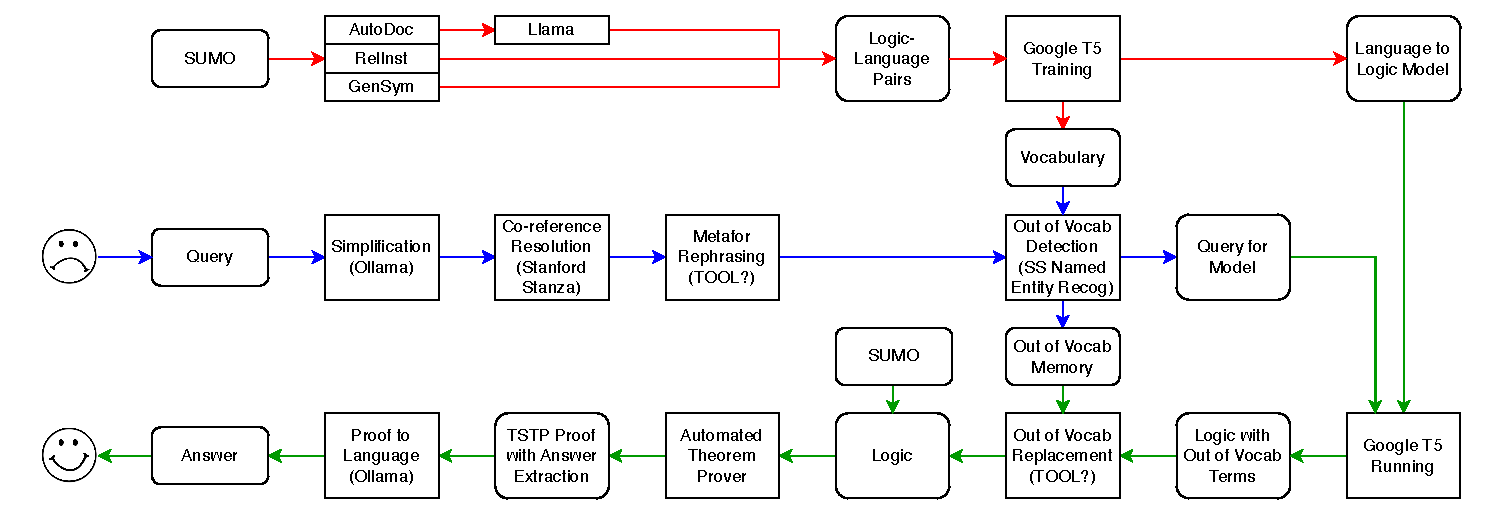
\includegraphics[width=\textwidth]{Architecture.pdf}
\caption{SUMO-ML-NLP architecture}
\label{ArchitecturePicture}
\end{figure}

In the training phase language-logic pairs are created, designed for training a machine learning 
system. 
Several approaches are used:

\begin{itemize}
\item build up sentences and logic expressions compositionally
\end{itemize}

\begin{itemize}
\item AutoDoc runs through all formulae in SUMO and generates natural language paraphrases,
      e.g., ADAM PLACE
\item Relation Instantion instantiates relations with arguments of appropriate types, then 
      generates natural language paraphrases from them, e.g., ADAM PLEASE.
\item Generation of Symbols builds up sentences and logic expressions compositionally, e.g.,
      ADAM PLEASE.
\item Google T5 Training
\end{itemize}

In the query preparation phase the query is reduced to simple unambiguous sentences; this query 
is used to illustrate the processing steps:
\emph{The nightmare hurricane Milton destroyed the beautiful bell pepper crop in western Florida, 
and it left many residents homeless. How did Milton affect Publix supermarkets?}
\begin{itemize}
\item Metaphor Rephrasing (using Ollama) rephrases the metaphor \emph{nightmare}, producing 
      \emph{The very bad hurricane Milton destroyed the beautiful bell pepper crop in western 
      Florida, and it left many residents homeless. How did Milton affect Publix supermarkets?}
\item Sentence Simplification removes the unnecessary adjectives \emph{very} and \emph{beautiful}, 
      and splits the sentence into two, producing \emph{Bad hurricane Milton destroyed the bell 
      pepper crop in western Florida. It left many residents homeless. How did Milton affect 
      Publix supermarkets?}
\item Co-reference Resolution (using the Stanford Stanza package) instantiates the \emph{It}, 
      producing \emph{Bad hurricane Milton destroyed the bell pepper crop in western Florida. 
      Hurricane Milton left many residents homeless. How did Milton affect Publix supermarkets?}
      This would have been complicated if \emph{it} had been omitted from the original sentence,
      which would still have been common natural language.
\item Out of Vocabulary Detection uses the Stanford Stanza Named Entity Recognition system to
      replaces the unknown names \emph{Milton} and \emph{Publix} with \texttt{UNK} tokens, 
      producing \emph{Bad hurricane \texttt{UNK\_OBJ\_1} destroyed the bell pepper crop in 
      western Florida. Hurricane \texttt{UNK\_OBJ\_1} left many residents homeless.
      How did \texttt{UNK\_OBJ\_1} affect \texttt{UNK\_OBJ\_2} supermarkets?}.
      The pairs \texttt{UNK\_OBJ\_1-Milton} and \texttt{UNK\_OBJ\_2-Publix} are recorded in the 
      Out of Vocabulary Memory.
\end{itemize}

In the query solving phase blah blah:
\begin{itemize}
\item Google T5 Running uses the language to logic model to produce SUO-KIF logic for the query,
      producing ADAM PLEASE.
\item Out of Vocabulary Replacement replaces the \texttt{UNK} tokens with the corresponding terms
      saved in the Out of Vocabulary Memory, producing ADAM PLEASE.
\item Automated Theorem Proving (ATP) combines the SUMO ontology with the logic generated from the
      query, converts it to the TPTP typed first-order logic (TFF) format~\cite{Sut23-IGPL},
      and runs an ATP system, e.g., Vampire~\cite{KV13}, producing a TSTP format~\cite{SZS04} 
      proof GEOFF PLEASE.
\item Proof to Language (using Ollama) is an an early prototype in our pipeline, which attempts 
      to COnvert the logical proof to a natural language answer.
\end{itemize}


\begin{verbatim}
(exists (?J ?C ?R)
  (and
    (instance ?J Human)
    (names "John" ?J)
    (instance ?C Climbing)
    (located ?C UNK-Region-1)
    (agent ?C ?J)))
\end{verbatim}

post processing (step 6) replaces the unknown term and asserts its type

\begin{verbatim}
(instance MtStHelens GeographicArea)

(exists (?J ?C ?R)
  (and
    (instance ?J Human)
    (names "John" ?J)
    (instance ?C Climbing)
    (located ?C MtStHelens)
    (agent ?C ?J)))
\end{verbatim}

%--------------------------------------------------------------------------------------------------
\section{Training the SUMO Model}
\label{Training}

ADAM

The compositional generation is potentially the most comprehensive. It consists of building ever more complex statements that wrap or extend simpler statements. Originally, this meant starting with a simple subject-verb-object but now encompasses a host of different constructs:

\begin{itemize}
\item six tenses (part, present, future and progressive or not) and correspond to SUMO expressions relative to a diectic 'Now'
\item  negation (for action sentences and separately for attitude wrappers that require higher-order logic, such as \texttt{believes}, \texttt{knows} etc)
\item  frequency-based selection of nouns and verbs
\item  human names and social roles
\item  restrict human actions with \texttt{CaseRole} of \texttt{agent} to be \texttt{IntentionalProcess}(es) and otherwise use the \texttt{CaseRole} of 'experiencer'
\item  use WordNet's noun and verb morphological exception lists
\item  counts of objects (0-10) are used randomly a small portion of the time, divided between using numerals some times and digits other times
\item  quantities of substances with units are used randomly a small portion of the time
\item  Some sentences have metric dates and times, in several formats
\item  Queries ('what','who') are generated sometimes, and with a question mark
\item  WordNet verb frames are used that index verbs to a context of use. However, this is quite limited compared to VerbNet and FrameNet, and still allows many semantically non-sensical sentences to be generated, while also missing some common sentence forms, especially use of prepositions
\item  Sentences with all variations of SUMO's \texttt{modalAttribute} are generated (\texttt{Possibility}, \texttt{Obligation} etc)
\item  Sentences with all variations of SUMO's \texttt{PropositionalAttitudes} are generated \texttt{believes},\texttt{knows},\texttt{says} etc
\item  Sentences with \texttt{says} have their content quoted
\item Imperative sentences with the English ``You (understood)'' form
\end{itemize}

%--------------------------------------------------------------------------------------------------
\section{Running a Query}
\label{Running}

GEOFF

%--------------------------------------------------------------------------------------------------
\subsection{Building the Query}
\label{BuildingQuery}

ROBERTO

JARRAD

ANGELOS

%--------------------------------------------------------------------------------------------------
\subsection{Answering the Query}
\label{AnsweringQuery}

ANGELOS

ADAM

%--------------------------------------------------------------------------------------------------
\section{Testing and Results}
\label{Testing}

RICHARD

TERRY 
%--------------------------------------------------------------------------------------------------
\section{Conclusion}
\label{Conclusion}

%--------------------------------------------------------------------------------------------------
\bibliographystyle{splncs04}
\bibliography{Bibliography.bib}
%--------------------------------------------------------------------------------------------------
\end{document}
%--------------------------------------------------------------------------------------------------
